\documentclass[a4paper,11pt,fleqn]{article}%fleqn pour aligner les equations à gauche
\usepackage{../../Styles/Exercice}

\newcommand{\chnum}{Chapitre 2}
\newcommand{\chtitle}{Analyse d'un système}
\newcommand{\dtype}{Exercices}
  
\begin{document}
\maketitle

\begin{multicols}{2}
\section{Spectre infrarouge}

\begin{enumerate}
    \item Nommer les molécules dont on a représenté les modèles moléculaires.
    \item Le spectre infrarouge représenté ci-dessous est celui d'une de ces molécules. Préciser laquelle en analysant la présence ou non de bandes caractéristiques.
\end{enumerate}
\begin{figure}[H]
    \centering
    \adjustbox{valign=b}{\subfloat[\textbf{Molécules à nommer}]{
    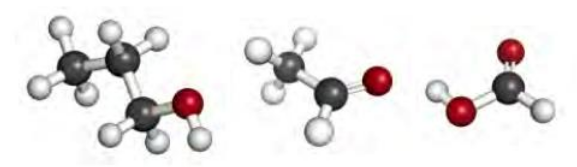
\includegraphics[scale=.5]{Ressources/TSPE_C2_Exercices_Fig1.png}}}
    \adjustbox{valign=b}{\subfloat[\textbf{Spectre IR de la molécule}]{
    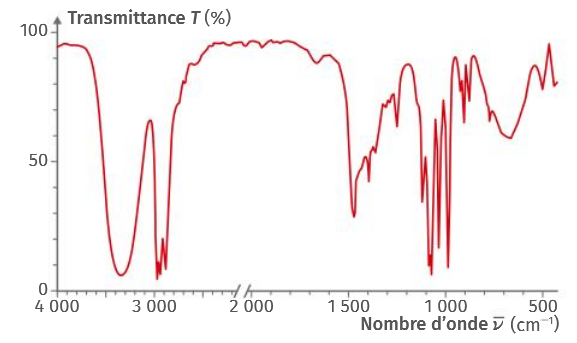
\includegraphics[scale=.35]{Ressources/TSPE_C2_Exercices_Fig2.png}}}
\end{figure}

\section{Famille des amides}
Le spectre infrarouge d'un composé organique X, de formule \ce{C3H7NO}, est donné ci-dessous. On rappelle que la liaison \ce{N}-\ce{H} donne une seule bande pour \ce{NH} et deux bandes pour \ce{NH2}.
\begin{enumerate}
    \item Repérer sur le spectre, les bandes caractéristiques des liaisons \ce{C}=\ce{O} et \ce{N}-\ce{H}.
    \item Le composé X est un amide, c'est-à-dire qu'il contient un enchaînement \ce{O}=\ce{C}-\ce{N}, possédant au moins une liaison \ce{N}-\ce{H}. Établir les formules demi-développées des trois molécules possibles de X.
    \item Parmi ces molécules, identifier X grâce à son spectre. Justifier le choix effectué.
\end{enumerate}
\begin{figure}[H]
    \centering
    \adjustbox{valign=b}{\subfloat[\textbf{Spectre IR de la molécule X}]{
    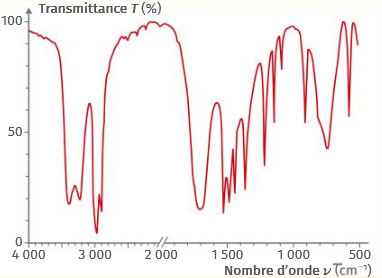
\includegraphics[scale=.6]{Ressources/TSPE_C2_Exercices_Fig3.png}}}
\end{figure}

\section{Détermination d'un conductivité}
On dispose d'une solution $S_1$ d'hydroxyde de sodium (\ce{Na+(aq)}; \ce{HO-(aq)}), de concentration $c_1$ = \SI{0,200}{\mole\per\liter} en soluté apporté.\\
Calculer la conductivité $\sigma$ de cette solution.\\

\noindent \colorbox{red!10}{
    \begin{minipage}{.95\linewidth}
    \textbf{Conductivités molaires ioniques à \SI{25}{\celsius} :}
    \begin{itemize**}
        \item $\lambda (\ce{Na+})$ = \SI{5,01E-3}{\siemens\meter\squared\per\mole}
        \item $\lambda (\ce{HO-})$ = \SI{19,8E-3}{\siemens\meter\squared\per\mole}
    \end{itemize**}
    \end{minipage}}

\section{Hydrolyse d'un ester}
On étudie la réaction d'hydrolyse de l'éthanoate d'éthyle, dont l'équation s'écrit : \begin{footnotesize}
$$\ce{C4H8O2(aq) + HO-(aq) ->}$$ $$ \ce{CH3COO-(aq) + CH3CH2OH(aq)}$$
\end{footnotesize}
\begin{enumerate}
    \item Nommer la famille de l'éthanoate d'éthyle.
    \item Sur le spectre IR, identifier deux bandes caractéristiques.
\end{enumerate}
\begin{figure}[H]
    \centering
    \adjustbox{valign=b}{\subfloat[\textbf{Spectre IR}]{
    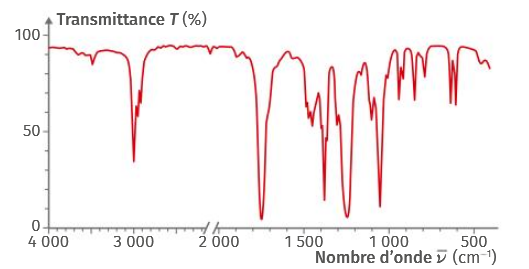
\includegraphics[scale=.5]{Ressources/TSPE_C2_Exercices_Fig4.png}}}
\end{figure}
On fait réagir une quantité $n_i$ d'hydroxyde de sodium (\ce{Na+(aq)}; \ce{HO-(aq)}) avec un large excès d'éthanoate d'éthyle. La conductance du mélange réactionnel est mesuré régulièrement et reportée ci-dessous :
\begin{table}[H]
    \centering \footnotesize
    \begin{tabular}{|>{\centering}m{1.8cm}|c|c|c|c|c|c|c|}
        \hline
        \textbf{Temps (s)} &  \num{0}&  \num{30}&  \num{60}&  \num{90}&  \num{120}&  \num{150} &  $t_{\infty}$\\
        \hline \textbf{Conductance G (\unit{\milli\siemens})} & \num{46,2}&  \num{18,6}&  \num{12,4}&  \num{12,3}&  \num{11,5}&  \num{10,8}&  \num{10,7}\\
        \hline
    \end{tabular}
\end{table}
\begin{enumerate}[resume]
    \item On constate que la conductance diminue au cours de la réaction. Justifier cette évolution.
    \item On appelle \emph{constante de cellule} le coefficient $k$ tel que $G=k\cdot \sigma$. Donner l'expression de la constante initiale $G_0$ en fonction de $k$, $n_i$, des conductivités molaires ioniques et de $V_T$, volume total du mélange. Trouver sa valeur dans le tableau.
    \item Déterminer de même l'expression de la conductance finale $G_f$. Relever sa valeur.
\end{enumerate}

\noindent \colorbox{red!10}{
    \begin{minipage}{.95\linewidth}
    \textbf{Conductivités molaires ioniques à \SI{25}{\celsius} :}
    \begin{itemize**}
        \item $\lambda (\ce{CH3COO-})$ = \SI{4,1E-3}{\siemens\meter\squared\per\mole}
        \item $\lambda (\ce{HO-})$ = \SI{19,8E-3}{\siemens\meter\squared\per\mole}
    \end{itemize**}
    \end{minipage}}

\section{Dosage par étalonnage}
Pour déterminer la concentration d'une solution d'iodure de potassium (\ce{K+(aq)}; \ce{I-(aq)}), on procède à un dosage par étalonnage en mesurant la conductivité $\sigma$ de plusieurs solutions d'iodure de potassium de concentrations connues.
\begin{table}[H]
    \centering \footnotesize
    \begin{tabular}{|>{\centering}m{2cm}|c|c|c|c|c|c|}
        \hline
        \textbf{Concentration $\mathbf{c}$ (\unit{\milli\mole\per\liter})} & \num{1,0}&\num{2,0}&\num{3,0}&\num{4,0}&\num{5,0}&\num{6,0}\\
        \hline
        \textbf{Conductivité $\mathbf{\sigma}$ (\unit{\milli\siemens\per\centi\meter})} & \num{3,43}&\num{6,85}&\num{10,3}&\num{13,7}&\num{17,2}&\num{20,6}\\
        \hline
    \end{tabular}
\end{table}
\begin{enumerate}
    \item Tracer la courbe $\sigma = f(c)$ à l'aide d'un tableur ou sur la calculatrice.
\end{enumerate}
On plonge la même cellule de mesure dans la solution à analyser. La conductivité mesurée est $\sigma$ = \SI{16,3}{\milli\siemens\per\centi\meter}.
\begin{enumerate}[resume]
    \item Déterminer la concentration de la solution analysée.
\end{enumerate}

\section{Diiode}
Le diiode \ce{I2(aq)} est une espèce chimique peu soluble dans l'eau. On procède au dosage par étalonnage d'une solution de diiode par spectrophotométrie.
\begin{table}[H]
    \centering \footnotesize
    \begin{tabular}{|c|c|c|c|c|}
        \hline
        \textbf{Concentration $\mathbf{c}$ (\unit{\micro\mole\per\liter})} & \num{50} & \num{250} & \num{750} & \num{1000}\\
        \hline\textbf{Absorbance (A)} & \num{0,041} & \num{0,220} & \num{0,703} & \num{0,872}\\
        \hline
    \end{tabular}
\end{table}
\begin{enumerate}
    \item Les mesures ont été obtenues à $\lambda$ = \SI{470}{nm}, longueur d'onde pour laquelle la molécule de diiode présente une absorbance maximale. En déduire la couleur de la solution de diiode.
    \item  À l'aide d'un tableur ou de la calculatrice, déterminer l'équation de la droite représentative de $A = f(c)$, modélisant la série de données.
    \item La solution de diiode analysée présente une absorbance $A$ = \num{0,514}. Déterminer sa concentration en quantité de matière.
\end{enumerate}

\section{Permanganate de potassium}
On dispose d'une solution de permanganate de potassium, de concentration approximativement égale à \SI{2}{\milli\mole\per\liter}. On souhaite connaître plus précisément cette concentration. On procède pour cela à un dosage par étalonnage à la longueur d'onde $\lambda$ = \SI{540}{nm}.

\begin{enumerate}
    \item Déterminer l'absorbance théorique de cette solution.
    \item Expliquer pourquoi on ne pourra pas déterminer avec fiabilité la concentration de la solution.
    \item Proposer une solution pour pallier ce problème.
\end{enumerate}
\noindent \colorbox{red!10}{
    \begin{minipage}{.95\linewidth}
    \textbf{Données :}
    \begin{itemize**}
        \item \textbf{Longueur de la cuve utilisée :} $l$ = \SI{1}{cm}
        \item \textbf{Gamme de mesure du spectrophotomètre :} \num{-0,97} < $A$ < \num{2,5}
        \item \textbf{Coefficient d'absorption molaire du permanganate de potassium à la longueur d'onde utilisée :} $\epsilon_{540~nm}$ = \SI{2,2E3}{\liter\per\mole\per\centi\meter}
    \end{itemize**}
    \end{minipage}}

\section{Dosage d'une gélule de guarana}
L'objectif de l'exercice est de déterminer le nombre de gélules de guarana pouvant être consommées quotidiennement sans risque. Pour déterminer la quantité de caféine présente dans une gélule, on réalise les expériences suivantes :
\begin{itemize}
    \item préparation d'une solution aqueuse $S_0$ de caféine de concentration $c_0$ = \SI{2,50}{\milli\mole\per\liter}
    \item préparation de six solutions filles à partir de la solution $S_0$ et mesure de leur absorbance
    \item dissolution d'une gélule de guarana dans \SI{500,0}{mL} d'eau distillée, dilution d'un facteur 10 de cette solution et mesure de l'absorbance de la solution diluée notée $S$ : $A$ = \num{0,524}
\end{itemize}
\begin{table}[H]
    \centering \footnotesize
    \begin{tabular}{|>{\centering}m{2cm}|c|c|c|c|c|c|}
        \hline
        \textbf{Solution} &$S_1$&$S_2$&$S_3$&$S_4$&$S_5$&$S_6$\\
        \hline
        \textbf{Concentration ($\times 10^{-2}$ \unit{\milli\mole\per\liter})} & \num{2,50} & \num{5,00} & \num{7,50} & \num{10,0}& \num{12,5}& \num{15,0}\\
        \hline\textbf{Absorbance} & \num{0,230} & \num{0,452} & \num{0,677} & \num{0,880}& \num{1,112}& \num{1,325}\\
        \hline
    \end{tabular}
\end{table}
\begin{figure}[H]
    \adjustbox{valign=b}{\subfloat[\textbf{Dose journalière}]{
    \begin{minipage}{.5\textwidth}
        Pour les adolescents, la dose journalière de caféine ingérable sans risque pour la santé est fixée à \SI{3}{\milli\gram} par kilogramme de masse corporelle.
    \end{minipage}}}
   \adjustbox{valign=b}{\subfloat[\textbf{Spectre UV-visible de la caféine}]{
    \centering
    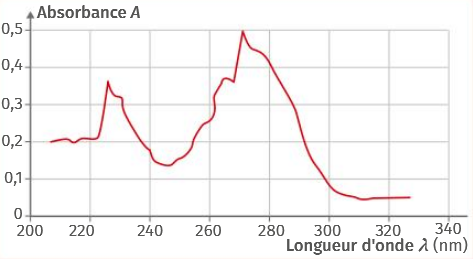
\includegraphics[scale=.6]{Ressources/TSPE_C2_Exercices_Fig5.png}}}
\end{figure}
\begin{enumerate}
    \item Préciser la longueur d'onde de travail
    \item Déterminer le nombre de gélules qu'un adolescent peut ingérer quotidiennement sans aucun risque sur sa santé
\end{enumerate}

\noindent \colorbox{red!10}{
    \begin{minipage}{.95\linewidth}
    \textbf{Donnée :}
    \begin{itemize**}
        \item \textbf{Masse molaire de la caféine :} $M$ = \SI{194,2}{\gram\per\mole}
    \end{itemize**}
    \end{minipage}}

    \section{Détermination d'une concentration}
    Dans un catalogue, on trouve deux références de soude, pour lesquelles on peut lire :
    
    \fbox{\begin{minipage}{.4\textwidth}
    \begin{large} \ce{NaOH(aq)}
    \end{large}
    \textbf{CAS : 1310-73-2}\\
    \textbf{M = \SI{40,02}{\gram\per\mole}}\\
    Pour dosage d'azote, bidon de \SI{5}{L}, \SI{32}{\percent}, $d$ = \num{1,35}\\
    Pur, Bidon de \SI{1}{L}, \SI{50}{\percent}, $d$ = \num{1,525}
    \end{minipage} }
    
    Calculer les concentrations en quantité de matière des deux solutions.
    
    \section{Titrage de l'acide chlorhydrique}
    On souhaite vérifier la concentration d'une solution d'acide chlorhydrique en réalisant un titrage avec suivi pH-métrique? Pour cela, le dosage d'un volume $V$ = \SI{20,0}{mL} de la solution de concentration $c$, inconnue par de la soude (\ce{Na+(aq)} ; \ce{HO-(aq)}) de concentration $c_B$ = \SI{1,00E-1}{\mole\per\liter} est réalisé.
    \begin{enumerate}
        \item Faire le schéma du montage.
        \item Écrire l'équation de la réaction acide-base qui se produit dans le bécher. 
    \end{enumerate}
    Les mesures de pH sont relevées dans ce tableau :
    \begin{scriptsize}
        \begin{tabular}{|>{\centering}m{0,4cm}|>{\centering}m{0,3cm}|>{\centering}m{0,3cm}|>{\centering}m{0,3cm}|>{\centering}m{0,3cm}|>{\centering}m{0,3cm}|>{\centering}m{0,4cm}|>{\centering}m{0,4cm}|>{\centering}m{0,4cm}|>{\centering}m{0,4cm}|>{\centering}m{0,4cm}|>{\centering\arraybackslash}m{0,4cm}|} \hline
    $\mathbf{V_B}$ & 0 & 2,0 & 4,0 & 6,0 & 8,0 & 10,0 & 12,0 & 14,0 & 16,0 & 18,0 & 18,5\\ \hline
    \textbf{pH} & 1,0 & 1,1 & 1,2 & 1,3 & 1,4 & 1,5 & 1,7 & 1,8 & 2,1 & 2,6 & 2,9\\ \hline 
    \end{tabular}\\
    \begin{tabular}{|>{\centering}m{0,4cm}|>{\centering}m{0,3cm}|>{\centering}m{0,3cm}|>{\centering}m{0,3cm}|>{\centering}m{0,3cm}|>{\centering}m{0,3cm}|>{\centering}m{0,4cm}|>{\centering}m{0,4cm}|>{\centering}m{0,4cm}|>{\centering}m{0,4cm}|>{\centering}m{0,4cm}|>{\centering\arraybackslash}m{0,4cm}|} \hline
    $\mathbf{V_B}$ & 18,8 & 19,0 & 19,2 & 19,5 & 19,8 & 20,0 & 21,0 & 22,0 & 23,0 & 24,0 & 25\\ \hline
    \textbf{pH} & 3,3 & 7,0 & 10,7 & 11,1 & 11,3 & 11,4 & 11,7 & 11,9 & 12,0 & 12,0 & 12,1\\ \hline 
    \end{tabular}
    \end{scriptsize}
    
    \begin{enumerate}[resume]
        \item Tracer la courbe $pH=f(V_B)$.
        \item Déterminer le volume à l'équivalence $V_E$.
        \item Exprimer puis calculer la concentration en quantité de matière en acide chlorhydrique.
    \end{enumerate}
    
    \noindent \colorbox{red!10}{\begin{minipage}{.47\textwidth}
        \textbf{Données :}\\
        \textbf{Couples acide-base :} \ce{H3O+(aq)}/\ce{H2O(l)} et \ce{H2O(l)}/\ce{HO-(aq)}
    \end{minipage}}
    
    \section{Simulation du titrage de l'ammoniaque}
    De nombreux produits ménagers contiennent de l'ammoniac \ce{NH3(g)} dissous. l'ammoniac est un gaz incolore, à l'odeur âcre et piquante, qui brûle les poumons et les yeux. Il faut donc utiliser ces solutions avec précautions.\\
    La solubilité de l'ammoniac est d'environ \SI{540}{\gram\per\liter} à \SI{20}{\celsius}. On souhaite représenter, en utilisant un langage de programmation, l'évolution des quantités de matière des espèces au cours du dosage d'une solution d'ammoniaque $S$ par l'acide chlorhydrique.
    \begin{enumerate}
        \item Calculer la concentration en (\unit{\mole\per\liter}) de la solution d'ammoniaque $S$ réalisée en dissolvant un volume $V_D$ = \SI{1,30}{L} d'ammoniac gazeux dans \SI{500}{mL} d'eau.
        \item Étudier la géométrie de la molécule d'ammoniac.
        \item Justifier la très grande solubilité de l'ammoniac.
    \end{enumerate}
    
    On réalise le titrage de $V$ = \SI{10,0}{mL} de solution avec une suivi conductimétrique par une solution d'acide chlorhydrique de concentration $c'$ = \SI{0,100}{\mole\per\liter}.\\
    On ajoute \SI{200}{mL} d'eau distillée avant de commencer pour éviter les phénomènes de dilution.
    
    \begin{enumerate}[resume]
        \item Légender le schéma du montage ci-dessous.
    \end{enumerate}
    \begin{center}
        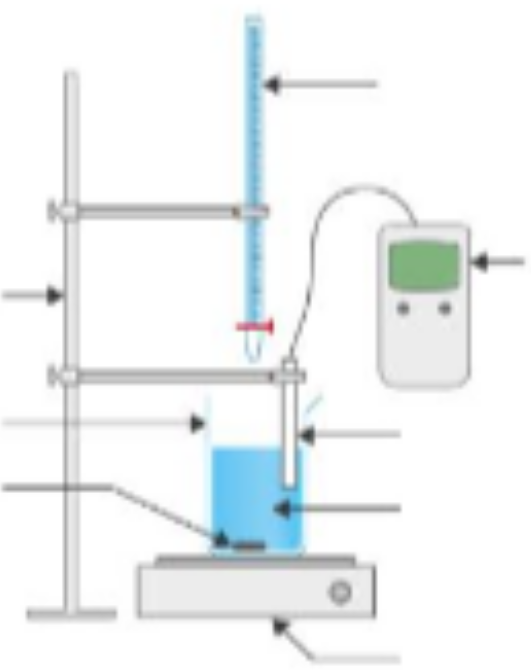
\includegraphics[scale=.28]{Ressources/TSPE_C3_Exercices_Fig3.png}
    \end{center}
    \begin{enumerate}[resume]
        \item Écrire l'équation de la réaction support du dosage.
        \item En considérant trois états (avant, pendant et après l'équivalence) étudier l'évolution des quantités de matière au cours du dosage.
        \item Définir l'équivalence du système.
        \item Programmer dans le langage Python, le calcul des quantités de matière et de la conductivité de la solution.
    \end{enumerate}
    
    \noindent \colorbox{red!10}{\begin{minipage}{.48\textwidth}
    \textbf{Données}
    \begin{itemize}
        \item \textbf{Volume molaire à \SI{20}{\celsius} :} $V_m$ = \SI{24,0}{\liter\per\mole}
        
        \item \textbf{Électronégativités :} $\chi(N)$ = 3,04, $\chi(H)$ = 2,20 et $\chi(O)$ = 3,44
        
        \item \textbf{Conductivités molaires ioniques :}\\
            $\lambda(\ce{H3O+})$ = \SI{35,0}{\milli\siemens\meter\squared\per\mole},\\
            $\lambda(\ce{HO-})$ = \SI{19,8}{\milli\siemens\meter\squared\per\mole}, \\
            $\lambda(\ce{NH4+})$ = \SI{7,36}{\milli\siemens\meter\squared\per\mole}, \\
            $\lambda(\ce{Cl-})$ = \SI{7,64}{\milli\siemens\meter\squared\per\mole}
        
        \item \textbf{Couples acide-base :} \ce{NH4+(aq)}/\ce{NH3(aq)} et \ce{H3O+(aq)}/\ce{H2O(l)}
    \end{itemize}
    
    \end{minipage}}
    
    
    \section{Dans une eau de brassage}
    En brasserie, les bières sont toutes produites selon le même procédé. Cependant, en fonction de l'utilisée, toutes ne possèdent pas les mêmes caractéristiques.\\
    On dose un volume $V_0$ = \SI{100}{mL} d'une eau de brassage par une solution de nitrate d'argent (\ce{Ag+(aq)} ; \ce{NO3-(aq)}) de concentration $c_2$ = \SI{10,0}{\milli\mole\per\liter}. L'équation de la réaction support du dosage est :
    $$\ce{Ag+(aq) + Cl-(aq) -> AgCl(s)}$$
    Déterminer si cette eau de brassage convient pour la fabrication d'une bière brune.
    
    \noindent \colorbox{red!10}{\begin{minipage}{.5\textwidth}
    \textbf{Différents types de bière}\\
    L'eau contient six principaux ions : les ions bicarbonate, sodium, chlorure, calcium, magnésium et sulfate. Leur proportion influence la douceur ou la dureté en bouche de la bière, mais aussi le processus de fabrication :
    \begin{itemize}
        \item la bière blonde, à l'eau douce : elle nécessite une eau peu minéralisée
        \item la bière ambrée, à l'eau riche en oligoéléments : cette eau doit contenir une forte proportion de sulfate de calcium (\num{70} à \SI{150}{\milli\gram\per\liter})
        \item la bière brune, à l'eau carbonatée : elle contient ne concentration importante en ion bicarbonate (\num{100} à \SI{300}{\milli\gram\per\liter}) et chlorure (\num{100} à \SI{200}{\milli\gram\per\liter})
    \end{itemize}
    \end{minipage}}
    
    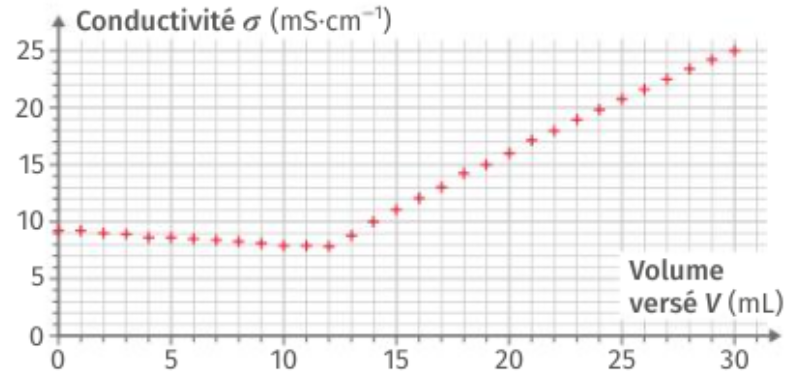
\includegraphics[scale=.33]{Ressources/TSPE_C3_Exercices_Fig2.png}
    
    \noindent \colorbox{red!10}{\begin{minipage}{.5\textwidth}
    \textbf{Données}
    \begin{itemize}
        \item \textbf{Conductivités molaires ioniques :}\\ $\lambda(\ce{Ag+})$ = \SI{6,190}{\milli\siemens\meter\squared\per\mole},\\ $\lambda(\ce{NO3-})$ = \SI{7,150}{\milli\siemens\meter\squared\per\mole}, \\ $\lambda(\ce{Cl-})$ = \SI{7,639}{\milli\siemens\meter\squared\per\mole}
        \item \textbf{Masse molaire du chlore :} $M(\ce{Cl})$ = \SI{35,5}{\gram\per\mole}
    \end{itemize}
    
    \end{minipage}}
    \section{Titrage de l'ibuprofène}
    L'ibuprofène est une molécule aux propriétés antalgiques, anti-inflammatoires et antipyrétiques; On souhaite vérifier la masse d'ibuprofène, noté \ce{R-COOH}, contenu dans un comprimé de \SI{400}{mg}.\\
    On dissout le comprimé dans une fiole jaugée contenant \SI{20}{mL} d'éthanol, solvant dans lequel l'ibuprofène est très soluble. On filtre la solution, ce qui permet d'éliminer les excipients (insolubles dans l'éthanol), puis on ajoute de l'eau distillée au filtrat. On considère que ce mélange eau-éthanol se comporte comme de l'eau.\\
    On réalise ensuite le titrage par suivi pH-métrique de cette solution par de la soude de concentration $c_B$ = \SI{0,20}{\mole\per\liter}. On relève les valeurs du pH pour chaque ajout de solution titrante. On entre les valeurs dans un tableur-grapheur et on utilise le logiciel pour faire afficher deux courbes $pH = f(V_B)$ et $\dfrac{dpH}{dV_B} = f(V_B$).
    
    %\begin{figure}[h!]
        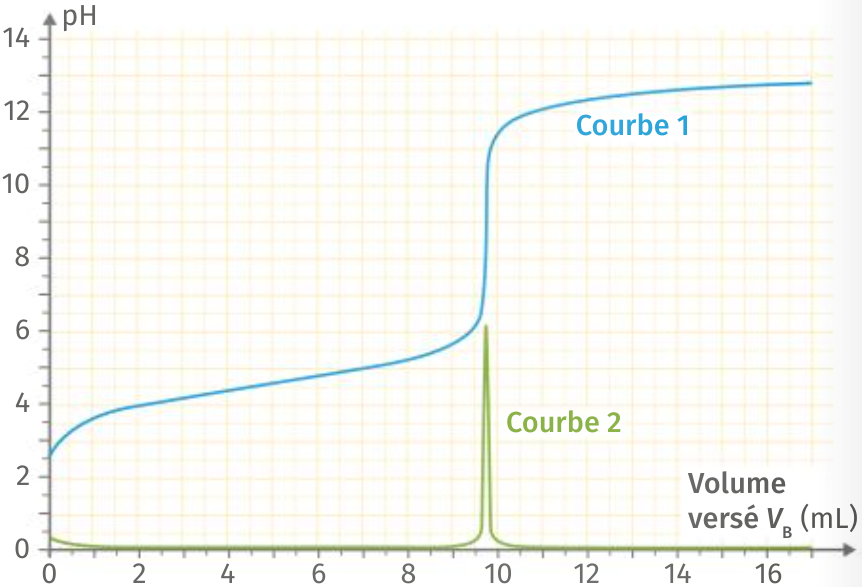
\includegraphics[scale=.28]{Ressources/TSPE_C3_Exercices_Fig1.png}
    %\end{figure}
    
    \begin{enumerate}
        \item En utilisant les données, calculer la masse maximale d'ibuprofène que l'on peut dissoudre dans \SI{40}{mL} d'eau. Préciser pourquoi on a ajouté de l'éthanol.
        \item Écrire l'équation de la réaction support du dosage.
        \item Identifier les courbes 1 et 2.
        \item Définir l'équivalence et établir la relation qui lie les quantités de matière à l'équivalence.
        \item Déterminer, en justifiant, le volume équivalent $V_E$.
        \item En déduire la masse d'ibuprofène dans le comprimé.
    \end{enumerate}
    \noindent\colorbox{red!10}{\begin{minipage}{.47\textwidth}
        \textbf{Données :}\\
        \textbf{Masse molaire de l'ibuprofène :} \\$M$ = \SI{206,0}{\gram\per\liter}\\
        \textbf{Solubilité de l'ibuprofène dans l'eau à \SI{37}{\celsius} :} \\$s$ = \SI{0,043}{\milli\gram\per\milli\liter}
    \end{minipage}}
\end{multicols}
\end{document}